\documentclass[aspectratio=169,11pt]{beamer}

\usetheme{Madrid}
\usecolortheme{default}
\usefonttheme{professionalfonts}
\setbeamertemplate{navigation symbols}{}

\usepackage[T1]{fontenc}
\usepackage[utf8]{inputenc}
\usepackage{lmodern}
\usepackage{booktabs}
\usepackage{tabularx}
\usepackage{array}
\usepackage{ragged2e}
\usepackage{tikz}
\usetikzlibrary{positioning}

\definecolor{irmsBlue}{HTML}{0A4585}
\definecolor{irmsGold}{HTML}{F4B400}
\definecolor{irmsLight}{HTML}{F3F6FA}
\definecolor{irmsText}{HTML}{1F2937}

\setbeamercolor{structure}{fg=irmsBlue}
\setbeamercolor{title}{fg=white,bg=irmsBlue}
\setbeamercolor{frametitle}{fg=white,bg=irmsBlue}
\setbeamercolor{block title}{fg=white,bg=irmsBlue}
\setbeamercolor{block body}{fg=irmsText,bg=irmsLight}
\setbeamercolor{itemize item}{fg=irmsBlue}
\setbeamercolor{normal text}{fg=irmsText,bg=white}

\setbeamertemplate{headline}{%
  \leavevmode
  \begin{beamercolorbox}[wd=\paperwidth,ht=1.95cm,dp=0.05cm,leftskip=0.2cm,rightskip=0.2cm]{title}
    \begin{minipage}[c][1.88cm][c]{0.11\paperwidth}
      \centering
      
\includegraphics[height=1.45cm]{../images/emblem.png}
    \end{minipage}
    \begin{minipage}[c][1.88cm][c]{0.76\paperwidth}
      \centering
      {\footnotesize\bfseries OFISI YA WAZIRI MKUU}\par
      {\small\bfseries TAWALA ZA MIKOA NA SERIKALI ZA MITAA}\par
      {\scriptsize TANGA, IRINGA, SINGIDA, MOROGORO, DODOMA, TABORA, LINDI NA MTWARA}\par
      {\normalsize\bfseries\color{irmsGold} MFUMO SHIRIKISHI WA USIMAMIZI WA MATOKEO (IRMS)}
    \end{minipage}
    \begin{minipage}[c][1.88cm][c]{0.11\paperwidth}
      \centering
      
\includegraphics[height=1.45cm]{../images/emblem.png}
    \end{minipage}
  \end{beamercolorbox}
}

\setbeamertemplate{title page}{
  \vspace*{1.9cm}
  \begin{beamercolorbox}[wd=\paperwidth,ht=2.5cm,dp=0.25cm,center]{title}
    {\LARGE\bfseries \inserttitle}\par
    \vspace{0.25cm}
    {\large \insertsubtitle}
  \end{beamercolorbox}
  \vspace{0.7cm}
  \begin{center}
    {\large \insertauthor}\par
    \vspace{0.2cm}
    {\normalsize \insertinstitute}\par
    \vspace{0.2cm}
    {\normalsize \insertdate}
  \end{center}
}

\title{MFUMO SHIRIKISHI WA USIMAMIZI WA MATOKEO (IRMS)}
\subtitle{Uwasilishaji wa Mkutano wa Kizoni: ACSEE, Utawala na Mwelekeo}
\author{Timu ya Mfumo wa IRMS}
\institute{PMO-RALG | Uendeshaji wa Mitihani}
\date{Februari 27, 2026}

\begin{document}

\begin{frame}
  \titlepage
\end{frame}

\begin{frame}{Malengo ya Uwasilishaji}
\begin{itemize}
  \item Kutoa uelewa wa pamoja wa mfumo wa IRMS kutoka mwanzo hadi mwisho.
  \item Kueleza mtiririko wa ACSEE: usajili, uingizaji alama, uhakiki, kufunga, kuhesabu, kuchapisha na tathmini.
  \item Kuonesha nguvu za mfumo katika udhibiti, uwajibikaji na kasi ya uamuzi.
  \item Kuonesha hali ya sasa ya utekelezaji kwa takwimu halisi za mfumo.
  \item Kupata maamuzi ya uongozi wa kanda kwa maboresho ya awamu inayofuata.
\end{itemize}
\end{frame}

\begin{frame}{Kwa Nini IRMS Ni Muhimu Kizoni}
\begin{block}{Changamoto ya Kiutendaji}
Mikoa, wilaya na shule zinahitaji utaratibu mmoja, unaodhibitika na unaoweza kuthibitishwa kisheria kwa matokeo.
\end{block}

\begin{columns}[T]
\column{0.5\textwidth}
\textbf{Bila IRMS}
\begin{itemize}
  \item Faili zilizotawanyika na marudio ya kazi
  \item Ucheleweshaji wa kufuatilia hitilafu
  \item Udhaifu wa ushahidi wa audit
  \item Uamuzi wa uchapishaji kuchelewa
\end{itemize}

\column{0.5\textwidth}
\textbf{Kwa IRMS}
\begin{itemize}
  \item Mzunguko mmoja wa kazi hadi matokeo
  \item Milango ya uhakiki kabla ya hatua inayofuata
  \item Rekodi za audit zenye ufuatiliaji kamili
  \item Uamuzi wa haraka wa utayari wa matokeo
\end{itemize}
\end{columns}
\end{frame}

\begin{frame}{Mnyororo Kamili wa Huduma za IRMS}
\begin{center}
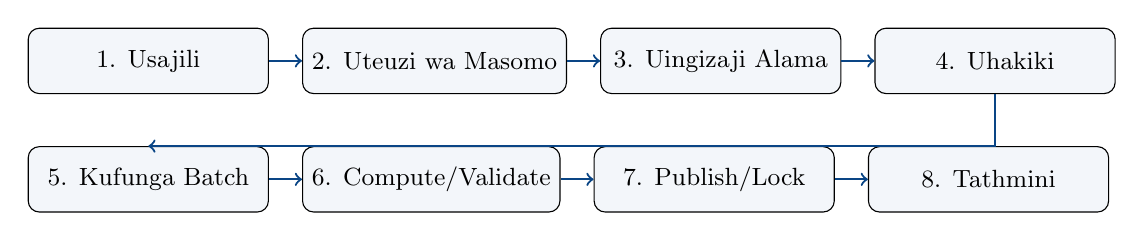
\begin{tikzpicture}[node distance=0.75cm, every node/.style={font=\small}]
  \node[draw, rounded corners, fill=irmsLight, minimum width=3.05cm, minimum height=0.83cm] (r1) {1. Usajili};
  \node[draw, rounded corners, fill=irmsLight, right=0.42cm of r1, minimum width=3.05cm, minimum height=0.83cm] (r2) {2. Uteuzi wa Masomo};
  \node[draw, rounded corners, fill=irmsLight, right=0.42cm of r2, minimum width=3.05cm, minimum height=0.83cm] (r3) {3. Uingizaji Alama};
  \node[draw, rounded corners, fill=irmsLight, right=0.42cm of r3, minimum width=3.05cm, minimum height=0.83cm] (r4) {4. Uhakiki};

  \node[draw, rounded corners, fill=irmsLight, below=0.66cm of r1, minimum width=3.05cm, minimum height=0.83cm] (r5) {5. Kufunga Batch};
  \node[draw, rounded corners, fill=irmsLight, right=0.42cm of r5, minimum width=3.05cm, minimum height=0.83cm] (r6) {6. Compute/Validate};
  \node[draw, rounded corners, fill=irmsLight, right=0.42cm of r6, minimum width=3.05cm, minimum height=0.83cm] (r7) {7. Publish/Lock};
  \node[draw, rounded corners, fill=irmsLight, right=0.42cm of r7, minimum width=3.05cm, minimum height=0.83cm] (r8) {8. Tathmini};

  \draw[->, thick, color=irmsBlue] (r1) -- (r2);
  \draw[->, thick, color=irmsBlue] (r2) -- (r3);
  \draw[->, thick, color=irmsBlue] (r3) -- (r4);
  \draw[->, thick, color=irmsBlue] (r4.south) |- (r5.north);
  \draw[->, thick, color=irmsBlue] (r5) -- (r6);
  \draw[->, thick, color=irmsBlue] (r6) -- (r7);
  \draw[->, thick, color=irmsBlue] (r7) -- (r8);
\end{tikzpicture}
\end{center}
\vspace{0.15cm}
\centering
\textbf{Kanuni kuu: kila hatua ina udhibiti kabla ya kuendelea mbele.}
\end{frame}

\begin{frame}{Muundo wa Teknolojia ya Mfumo}
\begin{columns}[T]
\column{0.52\textwidth}
\textbf{Msingi wa Teknolojia}
\begin{itemize}
  \item Laravel 12.48.1 na PHP 8.3
  \item Blade + Alpine.js upande wa mtumiaji
  \item Tailwind CSS 4 na Vite
  \item SQLite kama hifadhidata ya uendeshaji
  \item Filament v3 kwa usimamizi wa admin
\end{itemize}

\column{0.48\textwidth}
\textbf{Namna ya Ujenzi}
\begin{itemize}
  \item CRUD kwa master data
  \item Workflow kwa shughuli nyeti za mzunguko
  \item Policy/Gate kwa hatua za mamlaka
  \item Audit-centric kwa uwajibikaji
\end{itemize}
\end{columns}
\end{frame}

\begin{frame}{Moduli Kuu Zinazotumika Kizoni}
\small
\begin{tabularx}{\textwidth}{>{\RaggedRight\arraybackslash}p{3.1cm} X}
\toprule
\textbf{Moduli} & \textbf{Kazi na Thamani} \\
\midrule
Usajili & Usajili wa watahiniwa, shule na miaka ya mitihani kwa scope husika. \\
ACSEE Allocation & Uteuzi wa masomo kwa combination na private candidates. \\
Mark Entry & Uingizaji CSV/ZIP, validation, moderation, approval, lock/unlock. \\
Results Processing & Compute/validate, profile ya grading, publish/lock snapshot. \\
Tathmini & Matokeo kwa shule/wilaya/mkoa, ranking na outlier analysis. \\
Governance \& Backup & Audit trails, backup/restore na kumbukumbu za urejeshaji. \\
\bottomrule
\end{tabularx}
\end{frame}

\begin{frame}{Mtiririko wa Uingizaji Alama ACSEE}
\begin{enumerate}
  \item Chagua muktadha: mwaka, mkoa, wilaya, shule, somo.
  \item Pakua template rasmi la alama.
  \item Pakia alama (CSV/ZIP) kwenye batch ya awali.
  \item Endesha validation ya ubora wa data.
  \item Fanya moderation na kushughulikia hitilafu.
  \item Approve na lock batch kuwa tayari kwa compute.
\end{enumerate}

\begin{block}{Faida ya Utawala}
Mfumo huzuia kuendelea kwenye compute bila batch kupita milango ya uhakiki.
\end{block}
\end{frame}

\begin{frame}{Sheria za Ubora wa Data na Compute}
\begin{itemize}
  \item Alama za somo zina-normalize hadi 100 kwa paper weights zilizowekwa.
  \item Compute ya ACSEE hutumia rounding ya namba nzima.
  \item Max marks ya msingi: Paper 1/2 = 100, Paper 3 = 50 (isipokuwa ukisanidi tofauti).
  \item Irregular statuses (INC, ABS, X) zinahesabiwa kwa kanuni za kipaumbele.
  \item Readiness inategemea marks zilizopandishwa na kuthibitishwa, si uploads pekee.
\end{itemize}
\end{frame}

\begin{frame}{Usalama, Mamlaka na Uwajibikaji}
\begin{columns}[T]
\column{0.5\textwidth}
\textbf{Udhibiti wa Upatikanaji}
\begin{itemize}
  \item Role + scope based access
  \item Ulinzi wa ngazi ya mkoa/wilaya/shule
  \item Policy/Gate checks kwa hatua nyeti
  \item Password enforcement na user status control
\end{itemize}

\column{0.5\textwidth}
\textbf{Ushahidi wa Utendaji}
\begin{itemize}
  \item Login na action audit logging
  \item Moderation/Unlock ina sababu na mhusika
  \item Publish/Lock na Admin Unlock zina trace kamili
  \item Backup/Restore zina audit trail
\end{itemize}
\end{columns}
\end{frame}

\begin{frame}{Utawala wa Matokeo: Publish, Lock, Unlock}
\begin{itemize}
  \item Compute run huzalisha matokeo ya toleo lenye version.
  \item Publish na Lock ni hatua mbili tofauti kwa ukaguzi wa utawala.
  \item Lock inalinda matokeo yasibadilishwe kiholela.
  \item Admin unlock ipo kwa exceptions zilizoidhinishwa.
  \item Snapshot/version huwezesha historia inayoeleweka na kuthibitishwa.
\end{itemize}
\end{frame}

\begin{frame}{Hali ya Sasa ya Mfumo (Feb 27, 2026)}
\small
\begin{tabularx}{\textwidth}{>{\RaggedRight\arraybackslash}p{6.1cm} >{\RaggedLeft\arraybackslash}X}
\toprule
\textbf{Kiashiria} & \textbf{Idadi ya Sasa} \\
\midrule
Mikoa iliyopo kwenye mfumo & 8 \\
Wilaya zilizopo kwenye mfumo & 19 \\
Shule zilizosajiliwa & 93 \\
Watahiniwa kwenye master records & 11,168 \\
Usajili wa ACSEE (2026) & 11,168 \\
Uteuzi wa masomo ACSEE (2026) & 48,299 \\
Jumla ya mark-import batches ACSEE (2026) & 581 \\
Locked batches ACSEE (2026) & 551 \\
Active result runs (pending/in\_progress) & 0 \\
Result run ya mwisho (ID 30) & completed, 8,973/8,973 processed \\
\bottomrule
\end{tabularx}
\vspace{0.2cm}
\footnotesize Chanzo: snapshot ya hifadhidata ya mfumo tarehe 2026-02-27 03:26.
\end{frame}

\begin{frame}{Nguvu Kuu za IRMS kwa Kanda}
\begin{enumerate}
  \item \textbf{Ufuatiliaji kamili}: kila hatua inaonekana na ina historia.
  \item \textbf{Udhibiti wa mchakato}: moderation, lock na unlock za kisheria.
  \item \textbf{Ubora wa data}: validation na sheria za irregularities.
  \item \textbf{Uwezo wa kazi nyingi}: bulk imports na filtering ya scope.
  \item \textbf{Uwajibikaji}: audit logs kwa maamuzi na matukio yote nyeti.
\end{enumerate}
\end{frame}

\begin{frame}{Hatari Muhimu na Vipaumbele vya Maboresho}
\begin{itemize}
  \item Kuendelea kuoanisha role/permission checks kwenye controllers zote.
  \item Kuimarisha reliability ya result runs na ufuatiliaji wa operational jobs.
  \item Kuandaa mpango wa scale ya database kadri mzigo unavyoongezeka.
  \item Kuendelea kusafisha labels za UI ili kupunguza tafsiri potofu za takwimu.
  \item Kuimarisha SOP na mafunzo ya watumiaji wa mkoa/wilaya/shule.
\end{itemize}
\end{frame}

\begin{frame}{Mpango wa Siku 90 (Ngazi ya Kizoni)}
\small
\begin{tabularx}{\textwidth}{>{\RaggedRight\arraybackslash}p{1.5cm} >{\RaggedRight\arraybackslash}p{3.8cm} X}
\toprule
\textbf{Dirisha} & \textbf{Kipaumbele} & \textbf{Matokeo Yanayotarajiwa} \\
\midrule
0--30 & Lifecycle reliability hardening & Kupungua kwa runs zilizokwama na kuimarika kwa utayari wa compute. \\
31--60 & Authorization consistency pass & Kupunguza edge cases za ruhusa na kuongeza uaminifu wa udhibiti. \\
61--90 & Scale + reporting optimization & Ufanisi zaidi kipindi cha mzigo mkubwa na dashboard bora za zoni. \\
\bottomrule
\end{tabularx}
\end{frame}

\begin{frame}{Mambo Tunayohitaji kutoka Uongozi wa Kanda}
\begin{itemize}
  \item Uthibitisho wa SOP za exception handling (unlock/recompute/escalation).
  \item Uteuzi wa zonal super-users kwa mafunzo na msaada wa haraka.
  \item Ratiba ya mapitio ya utendaji (kila wiki wakati wa msimu wa mitihani).
  \item Idhini ya vipaumbele vya maboresho ya awamu inayofuata.
\end{itemize}

\vspace{0.35cm}
\centering
\Large\textbf{IRMS ipo tayari kuongezwa kwa kiwango kwa misingi ya utawala imara.}
\end{frame}

\begin{frame}{Kiambatisho: Nyaraka Zilizotumika}
\footnotesize
\begin{itemize}
  \item \texttt{docs/IRMS\_ADMIN\_PANEL\_ARCHITECTURE\_REPORT.md}
  \item \texttt{MARK\_ENTRY\_WORKFLOWS.md}
  \item \texttt{COMPLETE\_SYSTEM\_SUMMARY.md}
  \item \texttt{app/Http/Controllers/Api/Results/AcseeLifecycleApiController.php}
  \item Snapshot ya takwimu za mfumo kupitia \texttt{php artisan tinker} (2026-02-27).
\end{itemize}
\end{frame}

\begin{frame}
\centering
\Huge Asanteni Sana
\vspace{0.35cm}

\Large Maswali na Majadiliano
\end{frame}

\end{document}
